\documentclass[12pt]{article}

\usepackage{tikz}
\usepackage[margin=0.5in]{geometry}
\usetikzlibrary{patterns, decorations.pathreplacing}

\begin{document}
    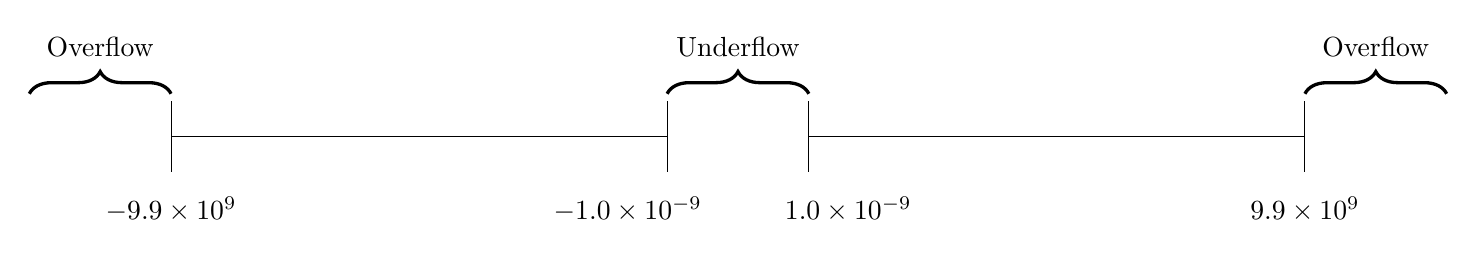
\begin{tikzpicture}[scale=0.9]
        \draw (-8,0) -- (-1,0);
        \draw (-8,-0.5) -- (-8, 0.5) node[black, below, yshift=-1.1cm]{$ -9.9 \times 10^9$};
        \draw (-1,-0.5) -- (-1, 0.5) node[black, below, yshift=-1.1cm, xshift=-0.5cm]{$ -1.0 \times 10^{-9}$};
        
        %\draw (0,-0.5) -- (0,0.5);

        \draw (1,0) -- (8,0);
        \draw (1,-0.5) -- (1,0.5) node[black, below, yshift=-1.1cm, xshift=0.5cm]{$ 1.0 \times 10^{-9}$};
        \draw (8,-0.5) -- (8,0.5) node[black, below, yshift=-1.1cm]{$ 9.9 \times 10^9$};
        
        \draw[
            very thick,
            decorate,
            decoration={
                brace,
                amplitude=8pt
            }            
        ] (-1,0.6) -- (1,0.6) node[black, midway, yshift=0.6cm]{Underflow};
        
        \draw[
            very thick,
            decorate,
            decoration={
                brace,
                amplitude=8pt
            }            
        ] (-10,0.6) -- (-8,0.6) node[black, midway, yshift=0.6cm]{Overflow};
        
        \draw[
            very thick,
            decorate,
            decoration={
                brace,
                amplitude=8pt
            }            
        ] (8,0.6) -- (10,0.6) node[black, midway, yshift=0.6cm]{Overflow};
        
    \end{tikzpicture}
\end{document}